\documentclass[UTF8]{ctexart}
\usepackage{subfiles}  

%下面的语句, 引入你的头部设置文件
\usepackage{C:/phpStorm_proj/02_myself_ID_EGO/+100_latex_all_math_sel/myPreamble} 
%必须是绝对路径,才能让各个tex在单独编译时使用到

\title{向量组的线性相关性}


%---------------------------------


\begin{document}
\tableofcontents % 生成目录
\date{} % 若不写这句, 则默认也会渲染出日期, 所以我们要手动赋空值
\maketitle  %这行代码, 让你前面的 title, author, date生效




\section{线性组合 linear combination}

\subsection{线性组合 : $\beta =k_1\alpha _1+k_2\alpha _2+...+k_n\alpha _n$ }

【线性组合】: \\
有 $ \beta, \alpha_1, \alpha_2, \alpha_n$, 它们都是n维向量. 若存在 $k_1, k_2, ..., k_n$这些系数(即权重), 能使得 $\beta =k_1\alpha _1+k_2\alpha _2+...+k_n\alpha _n$, 则就称 $\beta$ 是向量组$\alpha_1, \alpha_2, \alpha_n$的一个``线性组合", 或称 $\beta$ 可由向量组$\alpha_1, \alpha_2, \alpha_n$ 来``线性表示". \\

那么这组系数k, 可不可以全取0? 可以. 这样的话,  $\beta=0$ 了. \\


\begin{myEnvSample}
	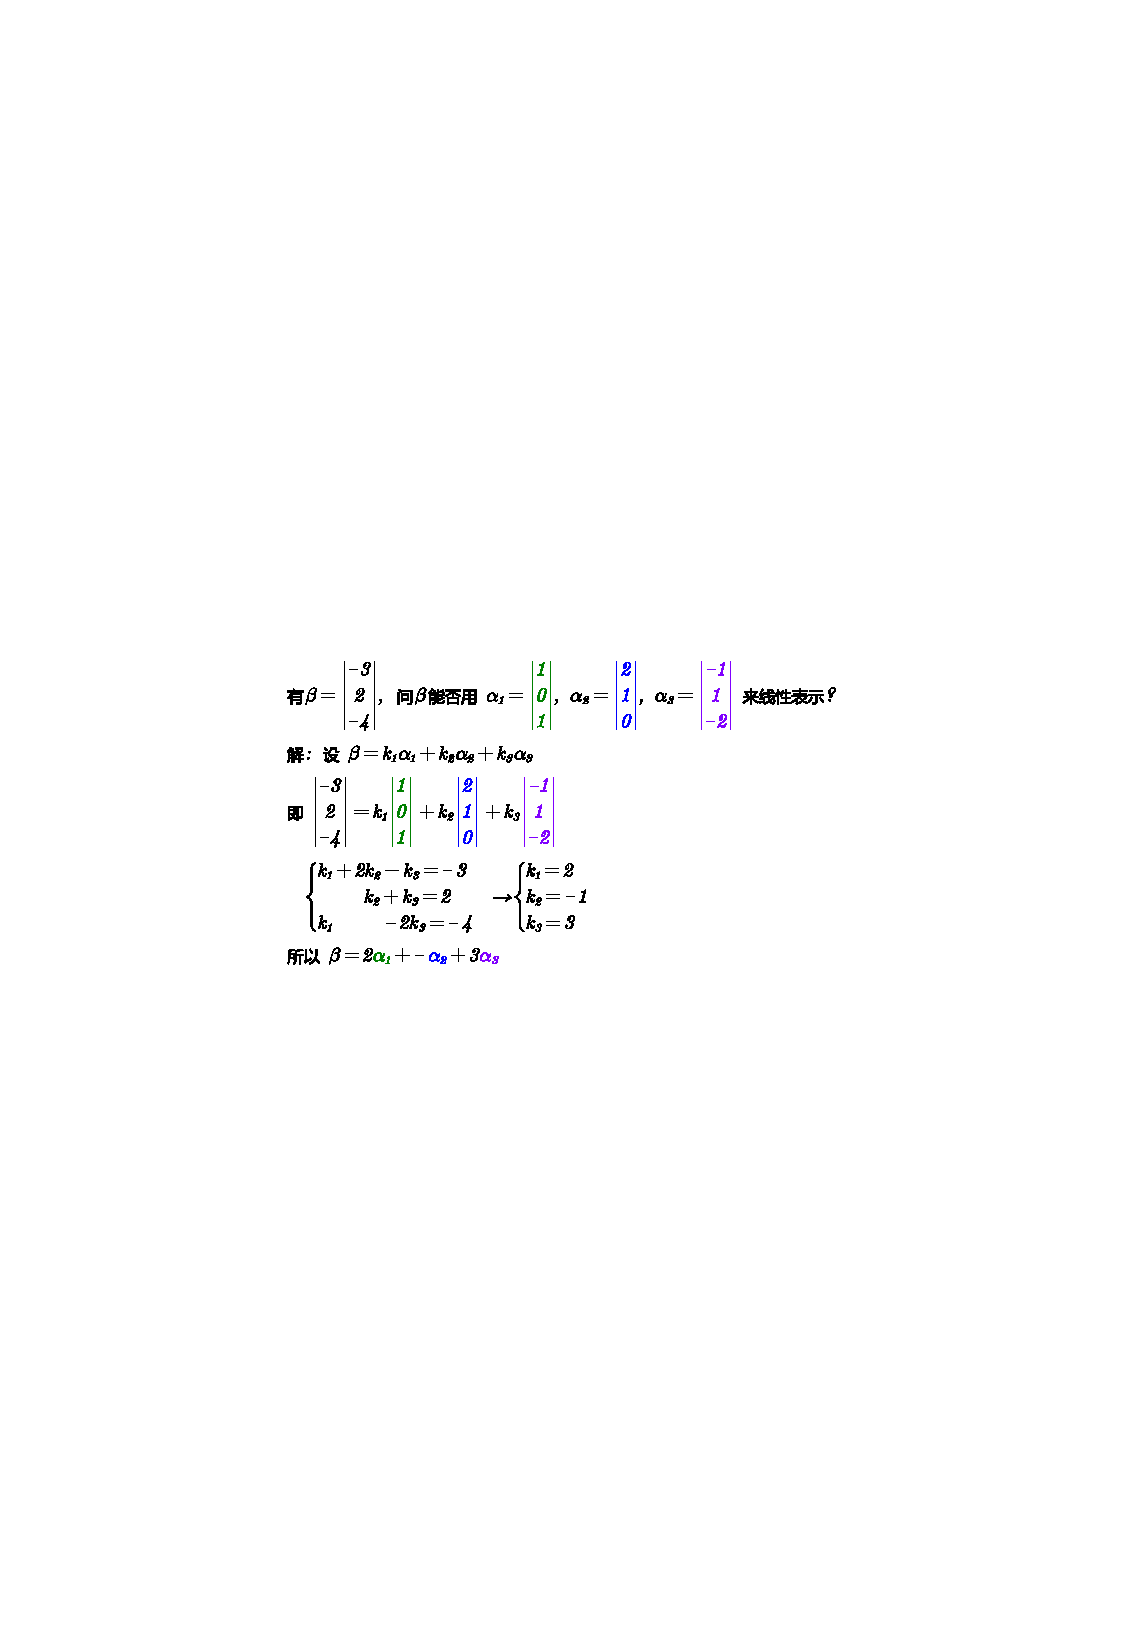
\includegraphics[width=0.75\textwidth]{img/0101.pdf}
\end{myEnvSample}



~\\
\hrule
~\\

\subsection{线性组合的性质}

\subsubsection{性质: 0向量, 可由任意向量组来表示. 即: $0\text{向量}=\ 0\alpha _1+0\alpha _2+...+0\alpha _n$}

~\\
\hrule
~\\

\subsubsection{性质: 向量组A中, 任取出其中的一个向量$α_i$出来, 它可以由这个向量组A来表示. 如: $\alpha _3=0\alpha _1+0\alpha _2+1\alpha _3...+0\alpha _n$}

~\\
\hrule
~\\

\subsubsection{任意一个向量组, 都可由这些个向量(即``n维单位向量")来表示: $\varepsilon _1=\left( 1,0,...,0 \right) ,\ \varepsilon _2=\left( 0,1,...,0 \right) ,\ ...\ ,\varepsilon _n=\left( 0,0,...,1 \right) $}

例如:$
\left| \begin{array}{c}
	1 \\
	2 \\
	3 \\
\end{array} \right|=1\left| \begin{array}{c}
	1 \\
	0 \\
	0 \\
\end{array} \right|+2\left| \begin{array}{c}
	0 \\
	1 \\
	0 \\
\end{array} \right|+3\left| \begin{array}{c}
	0 \\
	0 \\
	1 \\
\end{array} \right|
$\\

~\\
\hrule
~\\


\subsection{线性相关 and 线性无关}

\subsubsection{线性相关 and 线性无关 的几何意义}

见本章的 \hyperlink{超链接定位符}{``张成"}部分.



~\\
\hrule
~\\

\subsubsection{线性相关}

【线性相关 linearly dependent】: \\
对于n个m维的向量 $ \vec{v_1},  \vec{v_2}, ...  \vec{v_n}$, 若存在一组 k (系数, 倍数)不全为0, 使得 $ k_1  \vec{v_1} + k_2  \vec{v_2} + ... + k_n  \vec{v_n} = 0 $, 则称 $ \vec{v_1},  \vec{v_2}, ...  \vec{v_n}$ 是``线性相关"的.\\

\begin{myEnvSample}
	例如: 下面这三个向量, 是否线性相关?
	\begin{align}
		\left| \begin{array}{l}
			1 \\
			0 \\
		\end{array} \right|,\ \left| \begin{array}{l}
			0 \\
			1 \\
		\end{array} \right|,\ \left| \begin{array}{l}
			2 \\
			3 \\
		\end{array} \right|
	\end{align}
	
	那么就看下面这个式子, 是否能存在非零的系数 (只要有一个k是不为零的, 就满足了我们的条件)
	
	\begin{align}
		k_1\left| \begin{array}{l}
			1 \\
			0 \\
		\end{array} \right|+k_2\left| \begin{array}{l}
			0 \\
			1 \\
		\end{array} \right|+k_3\left| \begin{array}{l}
			2 \\
			3 \\
		\end{array} \right|=0
	\end{align}
	
	那么显然, 当 $ k_1$取2, $k_2$取3, $k_3$取1时, 该式子能成立. 即, 的确存在一组非零的k. \\
	这就说明, 这三个向量, 是``线性相关"的. (不需要所有的系数k都不为0, 只要有一个系数k不为零就行了.)
\end{myEnvSample}


若只能是 k全为0时, 该等式才成立, 那么这些向量 $ \vec{v_1},  \vec{v_2}, ...  \vec{v_n}$ 就是``线性无关"的 (linearly independent). \\

\textbf{``线性无关"就表示, 这组向量中的任何一个, 都无法表示成其他向量的``线性组合". 即, 它们中每一个向量, 都是``独当一面"的, 无法被其他向量所替代.}

~\\
\hrule
~\\

\subsubsection{线性无关}

不是线性相关, 就是``线性无关"了.

~\\
\hrule
~\\

\subsection{线性相关的 性质, 定理}

\subsubsection{向量组中, 若其中有两个向量成比例, → 则该向量组中的所有成员, 就都``线性相关".}

如:
\begin{align*}
	\underset{ \text{注意:\ 这两个向量成比例}}{\underbrace{(-1)\left| \begin{array}{l}
				1 \\
				2 \\
			\end{array} \right|+(-\frac{1}{2})\left| \begin{array}{l}
				2 \\
				3 \\
			\end{array} \right|}}+0\left| \begin{array}{l}
		5  \\
		19 \\
	\end{array} \right|+0\left| \begin{array}{l}
		-1 \\
		99 \\
	\end{array} \right|=0
\end{align*}

~\\
\hrule
~\\

\subsubsection{含有0向量的任一向量组, 必``线性相关".}

如:
\begin{align*}
	0\vec{v}_1+0\vec{v}_2+0\vec{v}_3+\underset{\text{随便取值}}{\underbrace{k}}\cdot \underset{\text{零向量}}{\underbrace{\vec{0}}}=0
\end{align*}

该向量组, 最后含有一个零向量, 该零向量前的k可以随便取值, 都不影响$k\vec{v}=\vec{0}$. 既然k可以随便取值, 那我们就有了一组不全为0的系数($k_1, k_2, ...k_n$) , 所以这些v向量, 就是``线性相关"的关系了. 

~\\
\hrule
~\\

\subsubsection{只有一个零向量, 则它必``线性相关".}

如:  $k\vec{0}=\vec{0}$ \\
k可以随便取值, 都不妨碍  $ k \cdot \vec{0}= \vec{0}$. 既然k可以随便取值, 那我们就有了一组不全为0的系数( $ k_1, k_2, ...k_n$) , 所以这些v向量(本例中只有一个向量), 就是"线性相关"的关系了.

~\\
\hrule
~\\



\subsubsection{一个向量 $\vec{v}$ , 线性相关的 充要条件是: 它本身就是零向量, 即 $\vec{v}=0$}

如: $k\vec{v}=\vec{0}$.  \\
k可以随便取值, 我们就有了一组不全为0的系数( $k_1, k_2, ...k_n]$ , 所以这些v向量, 就是``线性相关"的关系了. 

~\\
\hrule
~\\

\subsubsection{$	\alpha _1,...,\alpha _s$ ``线性相关" 的充要条件是: 至少一个向量, 可以由其余向量来表示}

~\\
\hrule
~\\

\subsubsection{$\alpha _1,...,\alpha _s$ 是``线性无关"的, 如果给它们再加一个向量$\beta$ , 即 $	\alpha _1,...,\alpha _s, \beta$ 变成了是``线性相关"的话, 则可以证明: $\beta$ 可由 $	\alpha _1,...,\alpha _s$ 来唯一的线性表示. }




~\\
\hrule
~\\

\subsubsection{若 $\vec{v_1}, ... \vec{v_r}$ 这组向量是"线性相关"的, 则给它们添加一些新的向量, \\它们整体($\vec{v_1}, ... \vec{v_r}, \vec{v_{r+1}}, ... \vec{v_s}$ ) 依然是"线性相关"的.}

证明过程, 如: \\
已知 $\vec{v_1}, \vec{v_2}, \vec{v_3}$ 是``线性相关"的, 即: \\
$k_1\vec{v}_1+k_2\vec{v}_2+k_3\vec{v}_3=0 $\\

把它扩充一下, 就有:\\
$(k_1\vec{v}_1+k_2\vec{v}_2+k_3\vec{v}_3) +(0\vec{v}_4+0\vec{v}_5)=0$\\

这5个系数k, 就是: $k_1, k_2, k_3, 0, 0$, 不全为0! 说明这组向量 $\vec{v_1}, ... \vec{v_5}$ 是``线性相关"的. 证毕.\\

即: 一个向量组中, 只要其中一部分向量是``线性相关"的, 则就可知道: 整个向量组中的全部向量, 都是``线性相关"的.\\
这里的本质就是: \textbf{比如一个队伍, 有1个女的, n个男的. 它满足``有女"性质. 之后无论往队伍里添加多少人, 它依然满足``有女"性质. 因为这个性质, 在最早的队伍中, 就已经被满足了.}\\


即:\\
部分``线性相关"$\overset{\text{能推导出}}{\rightarrow}$整体``线性相关'' \\
整体``线性相关"$\overset{\text{能推导出}}{\rightarrow}$部分``线性相关'' \\

同样就是说: \textbf{整体``无女"的话, 则其中的子集部分也``无女".}



~\\
\hrule
~\\

\subsubsection{在一个n维空间中, 存在m个n维向量的话, 并且是$m>n的$话,则这个向量组(即含有m个向量的), 一定是``线性相关"的. 即: n+1个n维向量, 一定``线性相关".}

比如, 在3维空间中, 存在4个三维的向量, 则由这4个向量所组成的``向量组", 一定是``线性相关"的. 即这个向量组中, 最多只有3个向量可以做基轴, 还有一个向量是多余的.



~\\
\hrule
~\\

\subsection{线性无关的 性质, 定理}


\subsubsection{任意一个非零向量, 必``线性无关".}

如: $k\vec{v}$. 因为 $\vec{v} \ne \vec{0}$, 则只能系数 k=0, 这样本例中, 我们就找不到一组不全为0的k, 那么这一向量必``线性无关".

~\\
\hrule
~\\

\subsubsection{(1)``线性无关"的向量组, 把每个向量的内部的维度, 往后接长, 则新的向量组, 依然是"线性无关"的. (2)``线性相关"的向量组, 把每个向量的内部的维度, 截短后, 则新的向量组, 依然是``线性相关"的.}


\begin{myEnvSample}
	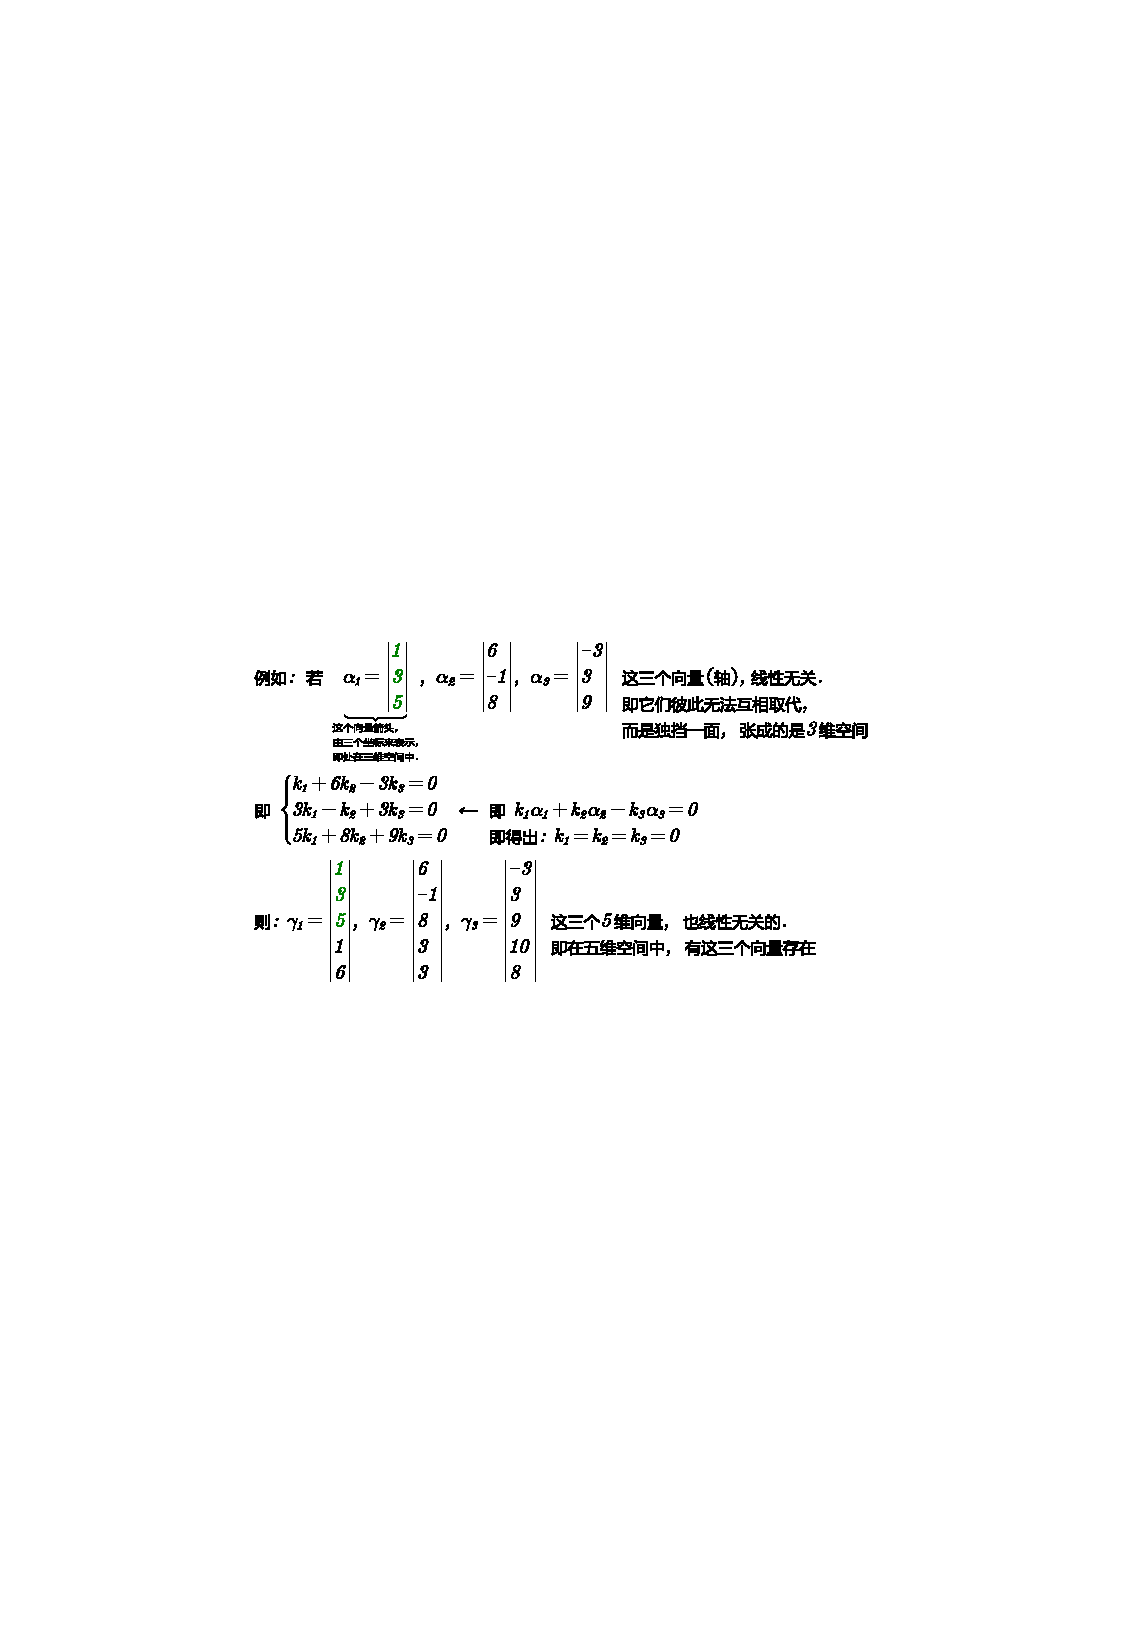
\includegraphics[width=0.9\textwidth]{img/0109.pdf}
\end{myEnvSample}


~\\
\hrule
~\\

\subsubsection{n个n维向量( 即,此处是``向量的个数"=``每个向量自己的维数")所构成的行列式, 则: (1) 若  $|D| \ne 0$, 则这些向量就是``线性无关"的. (2) 若 D=0, 则这些向量是``线性相关"的.}




\begin{myEnvSample}
	如: 这三个向量是``线性相关"还是``无关"的? 
	\begin{align*}
		\left| \begin{array}{l}
			1\\
			0\\
			3\\
		\end{array} \right|,\ \left| \begin{array}{l}
			2\\
			1\\
			1\\
		\end{array} \right|,\ \left| \begin{array}{l}
			1\\
			1\\
			0\\
		\end{array} \right|
	\end{align*}
	
	那么我们就来算算它们作为一个整体的行列式的值, 是否=0?
	\begin{align*}
		\left| \begin{matrix}
			1&		2&		1\\
			0&		1&		1\\
			3&		1&		0\\
		\end{matrix} \right| = ?
	\end{align*}
\end{myEnvSample}


~\\
\hrule
~\\

\subsubsection{n维的``单位向量"组 (单位向量, 显然就是``基轴"本身了), 是它们是``线性无关"的. }


~\\
\hrule
~\\

\subsubsection{替换定理:在线性空间中, 给出两个有限向量组: $a_1, a_2, ..., a_t$, 与 $b_1, b_2, ..., b_s$. 若向量组1是``线性无关''的,并且``向量组1"可由``向量组2"来线性表示的话,则:  $t \leq s$. }


向量组1中向量, 是``线性无关"的. 所以它的t轴(都属于基轴了), 彼此独立, 成为独当一面的维度. \\
向量组2中的向量, 可以用来表示向量1中的轴. 这就意味着, 向量组2中可能存在多余的``伪轴". 所以``向量组2"中的向量数量s, 一定是 $\geq$ ``向量组1"中的向量数量t的. \\



~\\
\hrule
~\\




\end{document}